\chapter{La Composition de services web}

\section*{Introduction}
\addcontentsline{toc}{section}{Introduction} \markboth{INTRODUCTION}{}

Dans ce chapitre, nous présentons dans un premier temps les %
définitions et les types de composition de services Web présents dans
la littérature. Ensuite, nous étudions

Enfin, un ensemble de travaux proposent des approches de la
composition dynamiques de services web sémantiques.

\newpage
\section{Définition et stratégies de composition}
\label{sec:defs}
Cette section a pour but d'exposer, d'une part, quelques définitions
et objectifs de la composition de services Web proposées par la
communauté\ref{sec:definitions}, et d'autre part, les différents types
et mécanismes de composition selon différents points de vue rencontrés
dans la littérature \ref{sec:proc-de-coord}, \ref{sec:types-de-composition}.

  \subsection{Définitions}
  \label{sec:definitions}
  Martin \emph{et al.} \cite{martin2004owl} définissent la composition
  comme étant \emph{``le processus de sélection, de combinaison et
    d'exécution de services en vue d'accomplir un objectif donné''}.\bigskip

  Selon S. Dustdar et W. Schreiner \cite{dustdar2005survey} : \emph{``
    L'infrastructure de base de services Web suffit pour la mise en
    œuvre d'interactions simples entre un client et un service Web. Si
    la mise en œuvre d'une application métier implique l'invocation
    d'autres services web, il est nécessaire donc de combiner les
    fonctionnalités de plusieurs services web. Dans ce cas, nous
    parlons d'une composition de services Web''}.\bigskip

  En d'autre terme, La composition de services Web désigne une
  opération qui consiste à construire de nouvelles applications ou
  services appelés \textbf{services composites} ou agrégats par
  l'assemblage ou l'agrégation de services existants nommés
  \textbf{services atomiques} ou élémentaires.\bigskip

  Medjahed \cite{medjahed2004thesis}de ça part a défini un service Web
  composite comme un \emph{``conglomérat de sous-traitance services
    Web (services appelés participants) travaillant en tandem pour
    offrir un service à valeur ajoutée.''}\bigskip

  La composition de services Web vise essentiellement quatre objectifs
  \cite{driss2011approche}:

  \begin{enumerate}
  \item Créer de nouvelles fonctionnalités en combinant de services
    déjà existants.
  \item Résoudre des problèmes complexes auxquels aucune solution\\
    n'a été trouvée.
  \item collaborer plusieurs entreprises ensemble.
  \item Optimiser et améliorer une fonctionnalité existante.
  \end{enumerate}

  \subsection{Cycle de vie d'une composition }
  \label{sec:cycle-de-vie}
  Comme l'illustre la figure \ref{fig:composition-life-cycle}, le
  cycle de vie de la composition de services Web comprend quatre
  phases \cite{sheng2014web}: la phase de \textit{définition}, La
  phase de \textit{sélection}, la phase de \textit{déploiement} et la
  phase d'\textit{exécution}:

  \begin{figure}[h]
    \centering
    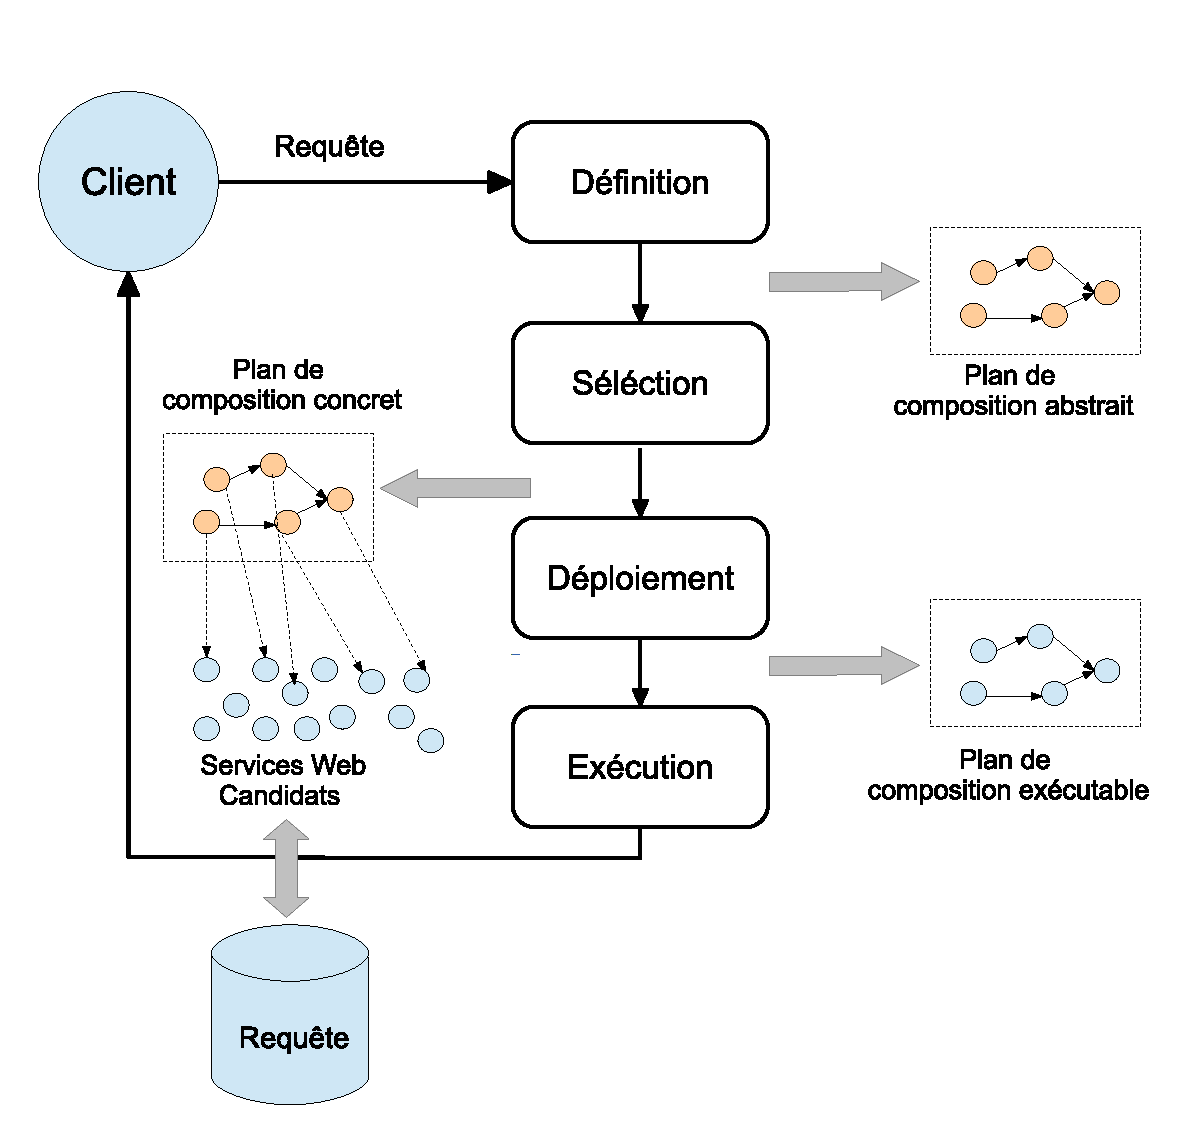
\includegraphics[width=0.9\textwidth]{figs/composition-life-cycle.eps}
    % TODO translate the figure
    % TODO reference the fig
    \caption{Cycle de vie d'une composition des services
      \cite{sheng2014web}.}
    \label{fig:composition-life-cycle.eps}
\end{figure}

%%% Local Variables:
%%% mode: latex
%%% TeX-master: "../main"
%%% End:


  \renewcommand{\descriptionlabel}[1]{\hspace{0.5cm}\textbullet~\textsf{#1}}
  \begin{description}
  \item[La phase de définition] Pendant cette phase, le client de
    service spécifie les exigence de composition de services en termes
    des besoins et des préférences pour le service
    composite. l'exigence est ensuite \textit{décomposé}, soit
    semi-automatique ou automatique, dans un modèle de
    \textbf{processus abstrait}(ce est à dire, le service composite
    abstraite), qui spécifie un ensemble d'activités, le contrôle et
    le flux de données entre eux, la qualité de service \acrshort{qos}
    et la gestion des exceptions.

    %% TODO: REWRITE
  \item[La phase de sélection.] Dans cette phase, pour chaque activité
    dans le service composite, les services Web appropriés qui
    répondent aux exigences de l'activité sont situés en cherchant sur
    le registre de service, sur la base des informations contenues
    dans les documents de description de service publiées. Il est
    probable que plus d'un service de candidat de répondre aux
    exigences. Par conséquent, le meilleur le service identifié doit
    être sélectionné. Après tous les services Web requis sont
    identifiés et liés aux activités correspondantes, le service
    composite construit est produite.

  \item[La phase de déploiement.]Dans cette phase, le service
    composite construit est déployé pour permettre son instantiation
    et l'invocation par les utilisateurs finaux. Le résultat de cette
    phase est le service composite exécutable.

  \item[La phase d'exécution.] Dans cette phase, l'instance de service
    composite est créé et exécuté par le moteur d'exécution, qui est
    aussi responsable de l'invocation des composants de service
    atomiques. Pendant l'exécution de l'instance de service composite,
    les tâches de surveillance, y compris le suivi d'exécution, mesure
    de la performance et la gestion des exceptions, doivent être
    effectuées.
  \end{description}
  \enddescription

  \subsection{Procédés de coordination}
  \label{sec:proc-de-coord}
  Nous distinguons deux méthodes utilisés pour décrire la composition
  de services dans un flot de processus métier: l'\emph{orchestration}
  de services et la \emph{chorégraphie} des services. Ces deux
  procédés de coordination décrivent deux aspects de création des
  processus métiers à partir de services Web composites
  \cite{peltz2003web}.\medskip

  \textbf{Un procédé} est représenté par un graphe orienté d'activités
  ou un flot de contrôle qui donne l'ordre d'exécution des activités
  et la logique de coordination de services. Chaque activité
  représente une fonctionnalité réalisée concrètement par un service
  \cite{chollet2009orchestration}.\medskip

  Il convient de noter que ces modèles ne sont pas utilisés
  exclusivement. En effet, une approche peut mettre en œuvre plus d'un
  procédé en même temps \cite{baryannis2010}.\medskip

  \newpage
  La figure \ref{fig:orchestration-vs-choregraphie} illustre ces deux
  approches en conjonction.

  \begin{figure}[h]
    \centering
    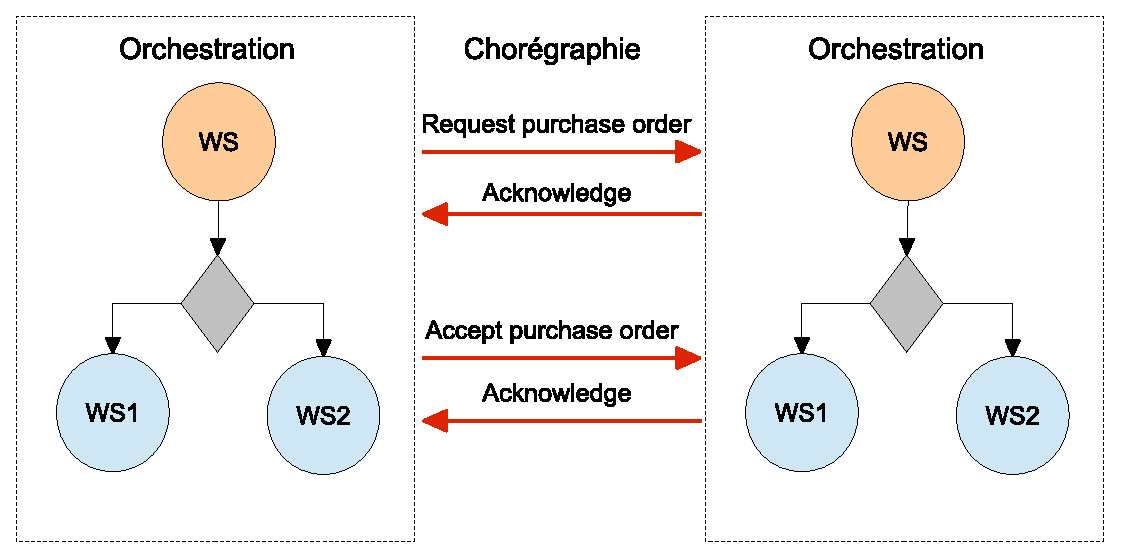
\includegraphics[width=1\textwidth]{figs/orchestration-vs-choregraphie.eps}
    \caption{Orchestration vs Chorégraphie selon Peltz
      \cite{peltz2003web}.}
    \label{fig:orchestration-vs-choregraphie}
\end{figure}

    \subsubsection{Orchestration}
    \label{sec:orchestration}
    Selon Sonia \emph{et al.} \cite{jamal2005environnement}:
    \emph{``L'orchestration de services Web permet de définir
      l'arrangement et l'enchaînement de ces services selon un
      canevas bien défini. Elle décrit la manière par laquelle les
      services peuvent interagir ensemble tout en incluant l'ordre
      d'exécution des différentes interactions''}.\bigskip

    Barros \emph{et al.} \cite{barros2006standards} définissent
    l'orchestration comme un ensemble de processus exécutés dans un
    ordre prédéfini afin de répondre à un but
    \cite{lopez2008selection}. Ce type de composition se base sur un
    procédé métier exécutable permettant de décrire d'enchaînement et
    les interactions des différents services basiques collaborant dans
    une composition.\medskip

    L'orchestration offre \textbf{une vision centralisée} de contrôle,
    le procédé est toujours contrôlé par l'un des partenaires
    métiers. Ce dernier joue le rôle d'un chef d'orchestre qui se
    charge d'appeler les services de la composition suivant l'ordre
    d'exécution déjà défini par le processus métier. Le principe de
    l'orchestration est illustré par La figure
    \ref{fig:orchestration}.

    \subsubsection{Chorégraphie}
    \label{sec:choregraphie-sec}
    Selon Sonia \emph{et al.} \cite{jamal2005environnement} : \emph{``
      La chorégraphie permet de tracer la séquence de messages
      échangés dans un contexte de composition de services Web. Elle
      est typiquement liée à la description de conversations
      existantes entre les services tout en impliquant plusieurs
      parties, incluant les clients, les fournisseurs et les
      partenaires''}.\bigskip

    D'après Barros \emph{et al.} \cite{barros2006standards}, la
    chorégraphie permet de décrire la composition comme un moyen
    d'atteindre un but commun en utilisant un ensemble de services
    Web. La collaboration entre chaque service Web de la collection
    (faisant partie de la composition) est décrite par des flots de
    contrôle \cite{lopez2008selection}.\medskip

    La chorégraphie offre \textbf{une vision décentralisée} et
    \textbf{globale} du système et exprime une vue d'ensemble des
    services interagissant dans le cadre d'une composition de
    services. Selon Peltz \cite{peltz2003web}, la chorégraphie
    illustre les différents échanges de messages entre les
    participants. Le principe de la chorégraphie est illustré par la
    figure \ref{fig:choregraphie}.

  \subsection{Stratégies de composition}
  \label{sec:types-de-composition}
  Un modèle de composition de service peut être relativement
  complexe. Il requiert la description et l'organisation de
  l'interaction entre les services et nécessite la gestion de
  plusieurs aspects comme les échanges de données entre les services,
  les pannes ou erreurs éventuelles, le contexte d'interaction, le
  degré d'automatisation des tâches, etc.\medskip

  Il existent une variété de spécifications, de langages et
  d'approches formelles développées par la littérature concernant la
  composition. Ces techniques sont également classés en fonction de
  différents dimensions, et selon les travaux effectués dans le champ
  de services web, les définitions des types de composition diffèrent
  d'une communauté de l'autre.\medskip

  Barros \emph{et al.} \cite{barros2006standards} classent la
  composition de services Web en trois catégories : la composition
  comportementale, l'orchestration et la chorégraphie, à l'instar de
  Barros \emph{et al.}, Peltz \cite{peltz2003web} considère que les
  deux dernières \textit{(orchestration, chorégraphie)}.\medskip

  \begin{figure}[h]
    \centering
    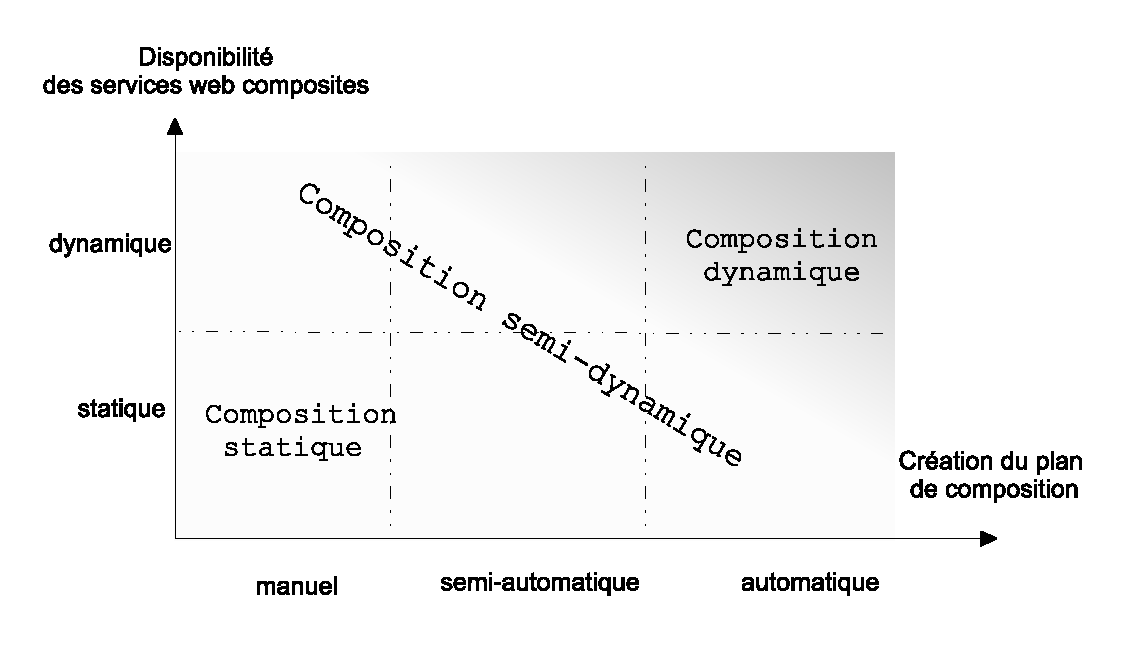
\includegraphics[width=1.1\textwidth]{figs/static-vs-dynamic-composition.eps}
    \caption{Classification des stratégies de composition
      \cite{fluegge2006challenges}.}
    \label{fig:static-vs-dynamic-composition}
\end{figure}
%%% Local Variables: 
%%% mode: latex
%%% TeX-master: "../main"
%%% End: 


  D'une autre façon, Fluegge \emph{et al.}\cite{fluegge2006challenges}
  dans une analyse de l'état de l'art considèrent l'orchestration et
  la chorégraphie comme des modèles d'exécution appliqués dans le
  contexte d'une composition. Il distingue trois stratégies de
  composition selon la disponibilité de services Web composites lors
  de composition et de le degré d'automatisation: composition
  \textbf{statique}, \textbf{semi-dynamique} et \textbf{dynamique}
  (voir la figure \ref{fig:static-vs-dynamic-composition}).

    \subsubsection{Composition statique/dynamique}
    \label{sec:comp-stat}
    Selon la disponibilité de services composites, La composition de
    services Web peut être soit une composition statique soit une
    composition dynamique \cite{driss2011approche}:\bigskip

    \renewcommand{\descriptionlabel}[1]{\hspace{0.5cm}\textbullet~\textsf{#1}}
    \begin{description}
    \item[Composition statique] :est appelé aussi composition
      \textit{off-line}, pré-compilée ou encore proactive. c'est une
      composition qui utilise de services basiques qui sont au
      préalablement définis d'une façon figée et qui ne peuvent pas
      changer en fonction du contexte du client. Ce type de
      composition engendre des applications peu flexibles, parfois
      inappropriées avec les exigences des clients.

    \item[Composition dynamique]: appelée aussi composition
      \textit{online}, post-compilée ou encore réactive. Elle se réfère
      à la sélection de services basiques à la volée. Autrement dit,
      la sélection de services basiques ne peut pas être définie à
      l'avance mais elle sera faite au moment de l'exécution en
      fonction des contraintes imposées par le client. Ceci permet d'
      élaborer différents scénario de composition qui offrent les
      mêmes fonctionnalités et qui tiennent compte de la dynamique de
      la situation du client.
    \end{description}
    \enddescription

    \subsubsection{Composition manuel/automatique}
    \label{sec:comp-manu}
    Selon le degré d'automatisation, nous distinguons:

    \renewcommand{\descriptionlabel}[1]{\hspace{0.5cm}\textbullet~\textsf{#1}}
    \begin{description}
    \item[Composition manuel]: Suppose que l'utilisateur gère la
      composition avec sa main, via un éditeur de texte et sans l'aide
      d'outils dédiés.

    \item[Composition semi-automatique]: C'est un pas en avant en
      comparaison avec la composition manuelle, dans le sens qu'elle
      fait des suggestions sémantiques pour aider à la sélection des
      services Web dans le processus de composition.

    \item[Composition automatique]: La composition automatique (ou
      encore dynamique selon \cite{fluegge2006challenges}) permet un
      développement plus rapide des applications à base de
      services. Elle consiste à préciser la requête d'un utilisateur
      sous forme d'objectifs à satisfaire. Un moteur de composition
      \textit{``intelligent''} choisit la combinaison de services
      répondant à l'objectif décrit. Il génère la composition de
      service adéquate de manière transparente à l'utilisateur. Ce
      principe a interpellé plusieurs communautés de recherche
      travaillant dans le domaine de l'intelligence artificielle.
      \cite{elie2010}
    \end{description}
    \enddescription

\section{Langages pour la composition}
\label{sec:lang-de-comp}
Afin de supporter la composition de services Web, plusieurs langages
de composition de services ont été proposés pour décrire et mettre en
oeuvre une composition. Dans cette section nous allons a faire un tour
d'horizon de quelques standards et langages principaux rencontrés dans
la littérature.

  \subsection{BPEL}
  \label{sec:bpel}
  \acrshort{bpel} est une spécification du consortium OASIS
  \footnote{\url{https://www.oasis-open.org}} issue de la fusion des
  spécifications \acrshort{xlang} Microsoft et \acrshort{wsfl} d'IBM ,
  il hérite les caractéristiques d'un langage structuré en blocs de
  \textsc{XLANG}, ainsi que les caractéristiques d'un graphe direct de
  \acrshort{wsfl} \cite{driss2011approche}.\medskip

  \textsc{BPEL} \textit{(appelé aussi \acrshort{bpel4ws} ou
    \acrshort{ws-bpel})} est le langage d'\textbf{orchestration} le
  plus utilisé dans l'industrie permettant la coordination des
  interactions entre l'instance du service composite et ses
  partenaires sous forme d'un schéma \acrshort{xml} \textit{(le script
    d'orchestration)}, il définit le processus, l'enchaînement et
  l'ordonnancement des actions qui seront exécutées par le moteur
  d'orchestration, agissant comme une machine virtuelle capable
  d'exécuter \textbf{le procédé métier} interprétable de
  \textbf{coordination} \cite{chollet2009orchestration}.\medskip

  \textsc{BPEL} repose sur un modèle constitué d'activités de
  coordination qui peuvent être de deux types, les activités de base
  ou élémentaires comme l'invocation (invoke) d'un service, l'attente
  d'une réponse et la génération d'une réponse (\verb|reply|), et les
  activités composites permettant du contrôle du flot de données comme
  les séquences (\verb|sequence|), les exécutions en parallèle
  (\verb|flow|) et les branchements (\verb|switch|, \verb|if|).

  \subsection{WS-CDL}
  \label{sec:WS-CDL}
  \acrshort{ws-cdl} \footnote{\url{http://www.w3.org/TR/ws-cdl-10/}}
  \cite{kavantzas2005web} est un langage de composition de services de
  type \textbf{chorégraphie} qui permet de décrire une vision
  \textbf{globale} des collaborations entre les services Web
  \cite{elie2010}, à l'instar des standards de services Web,
  \textsc{WS-CDL} est basé sur \textsc{XML}, il complète la
  description \acrshort{wsdl} de services Web afin de décrire les
  points d'interactions entre les services Web engagés dans une
  composition. Contrairement à la spécification \textsc{BPEL}
  \ref{sec:bpel}, Les interactions de services sont décrites d'une
  manière \textit{peer-to-peer}, Il n'y a pas de notion de
  coordination ou d'un service Web principal d'orchestration.\medskip

  \textsc{WS-CDL} reprend et développe la spécification
  \acrshort{wsci} \footnote{\url{http://www.w3.org/TR/wsci/}}
  \cite{arkin2002web} décrivant les séquences ordonnées de messages
  impliquant plusieurs entités (services Web) engagés dans une
  composition visant à accomplir un objectif commun, il permet de
  décrire les règles selon lesquelles une collaboration doit avoir
  lieu par le biais d'un fichier \textsc{XML} décrivant une
  chorégraphie.

  \subsection{WSMF}
  \label{sec:wsmf}
  \acrshort{wsmf} \cite{fensel2002web} est un initiative européen pour
  fournir une plate-forme riche de modélisation décrivant plusieurs
  aspects de services web. Son objectif principale est de permettre le
  commerce électronique (\emph{E-commerce}) par l'application de web
  sémantique aux services Web.  Le standard \acrshort{wsmf} est centré
  autour de deux principes complémentaire \cite{baryannis2010}: un
  découplage fort de différents aspects des applications de
  \textit{E-commerce}, et des mécanismes de médiation permettant un
  dialogue automatique entre les différents composants.\medskip

  \acrshort{wsmf} comprend quatre éléments principaux:

  \SpecialItem
  \begin{itemize}
  \item Des ontologies qui fournissent la terminologie utilisée par
    les autres éléments.

  \item Un répertoire d'objectifs qui définit les problèmes qui
    doivent être résolus par les Web services.

  \item Des descriptions des Web services qui définissent les
    différents aspects liés aux Web services

  \item Des médiateurs qui sont en charge des problèmes
    d'interopérabilité.
  \end{itemize}
  \enddescription

  Il y a deux principaux projets en WSMF : \textsc{SWWS} et
  \textsc{WSMO}, le standard \textsc{SWWS} fournit un cadre de
  description, la découverte et la médiation pour les services Web,
  tandis que l'ontologie de service \textsc{WSMO} inclut des
  définitions pour les objectifs, les médiateurs et les services Web.

  \subsection{OWL-S}
  \label{sec:owl-s}

  \begin{figure}[h]
    \centering
    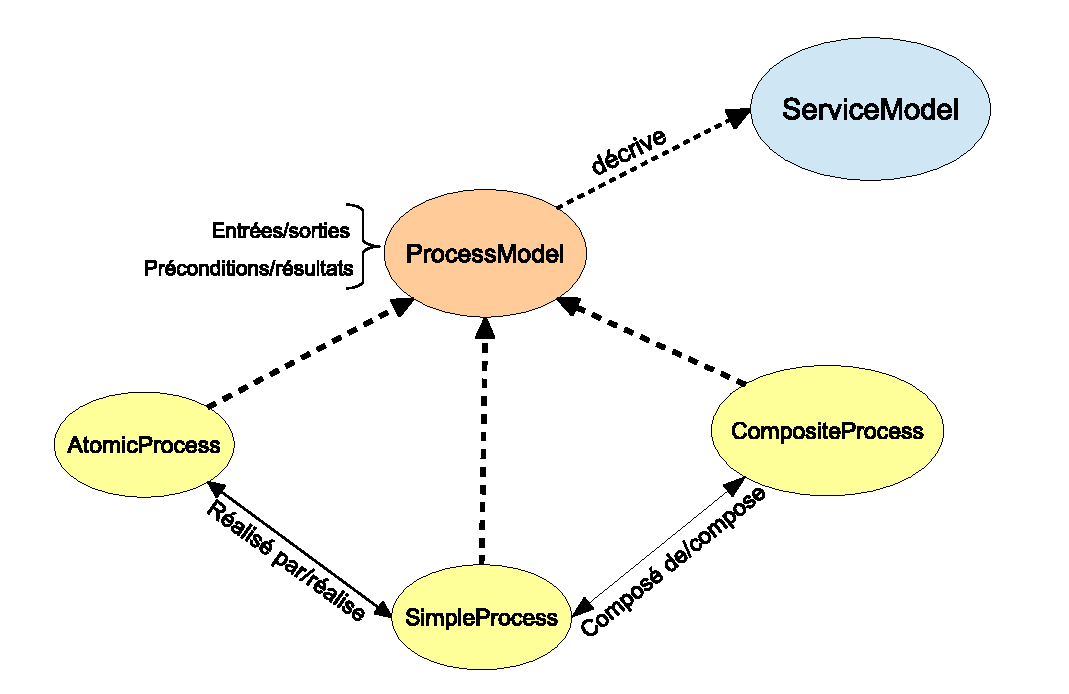
\includegraphics[width=0.95\textwidth]{figs/owls-processModel.eps}
    \caption{Les éléments d'une ontologie ProcessModel}
    \label{fig:owls-processModel}
\end{figure}
%%% Local Variables:
%%% mode: latex
%%% TeX-master: "../main"
%%% End:

  \textsc{OWL-S} définit une sous-classe de \verb|ServiceModel|
  appelée \verb|ProcessModel|. elle est utilisé pour décrire le
  service comme un processus. Le modèle de processus identifie trois
  types de processus illustrés dans la figure
  \ref{fig:owls-processModel}:

  \renewcommand{\descriptionlabel}[1]{\hspace{0.5cm}\textbullet~\textsf{#1}}
  \begin{description}
  \item[Le processus atomique]: (\verb|AtomicProcess|) directement
    invoqué par l'intermédiaire d'un \verb|ServiceGrounding|

  \item[Le processus composé]: (\verb|CompositeProcess|) décomposable
    en d'autres processus plus simples en utilisant les commandes de
    contrôle (par exemple: \textit{if/else, sequences} etc.

  \item[Le processus simple]: (\verb|SimpleProcess|) non-invoquable,
    il fournit simplement une vue d'un processus atomique ou une
    représentation simplifié d’un processus composé.
  \end{description}
  \enddescription

  Dans \cite{martin2004owl}, les auteurs discute les avantages de la
  description de service plus riche soutenue par \textsc{OWL-S}. il
  décrit comment \textsc{OWL-S} est utilisé dans le contexte d'autres
  standards, telles que \textsc{WSDL}, \textsc{UDDI} et \textsc{BPEL}.

  \subsection{Comparaison}
  \label{sec:langs-comparaison}
  Une composition de services Web nécessite la satisfaction de
  plusieurs exigences techniques \cite{sheng2014web,
    bucchiarone2006survey} , le tableau
  \ref{comparaison-des-standards-et-langages-d-composition} montre une
  comparaison entre les langages et standards étudiées dans cette
  section selon les critères suivants:

  \begin{table}[htb!]
  \centering
  \begin{tabular}{|lcccc|}
    \hline
    \head{Langages}& \textsc{BPLE} & \textsc{WS-CDL} & \textsc{WSFM} & \textsc{OWL-S}\\
    \hline\hline
    \textbf{Composabilité} &\verb|+|& \verb|+|&\verb|-|&\verb|+|\\
    \textbf{Representation du rôle} &\verb|+|& \verb|+|&\verb|-|&\verb|-|\\
    \textbf{Support des structures complexes} &\verb|+|& \verb|+|&\verb|-|&\verb|+|\\
    \textbf{Compensabilité} &\verb|+|& \verb|+|&\verb|-|&\verb|-|\\
    \textbf{Support du sémantique} &\verb|-|& \verb|-|&\verb|+|&\verb|+|\\
    % TODO réviser critères
    \textbf{Support industriel} &\verb|+|& \verb|-|&\verb|-|&\verb|+|\\
    \hline
  \end{tabular}
  \newline

  \raggedright
  (\verb|+|) support, (\verb|-|) pas du support.
  \caption{Comparaison des standards et langages de composition}
  \label{comparaison-des-standards-et-langages-d-composition}
\end{table}
%%% Local Variables:
%%% mode: latex
%%% TeX-master: "../main"
%%% End:


  \renewcommand{\descriptionlabel}[1]{\hspace{0.5cm}\textbullet~\textsf{#1}}
  \begin{description}
  \item [La composabilité] indique la capacité d'assembler de services
    participants dans un processus de composition et de modéliser les
    interactions entre eux.

  \item [La representation du rôle] indique La représentation de rôle
    indique la capacité de refléter la le comportement que le
    participant doit présenter afin d'interagir dans le processus de
    composition.

  \item [Le support des structures complexes] la capacité de modéliser
    les structures complexes qui reflètent les règles des actions
    réalisées dans le processus de composition logique d'exécution et
    de commande.

  \item [Compensabilité] est la capacité de gérer les exceptions de
    processus lors de l'exécution du processus de composition

  \item [le support du sémantique] est la capacité de représenter la
    sémantique de services participants pour faciliter la découverte
    de services et la composition dynamique.

  \item [le support industriel] indiqué par la qualité des outils et
    le support industriel de la technologie.
  \end{description}
  \enddescription

  D'après le tableau
  \ref{comparaison-des-standards-et-langages-d-composition} Nous
  pouvons constater que tous les langages sauf \textsc{WSMF}
  supportent la modélisation des structures complexes. seulement
  \textsc{BPEL} et \textsc{WS-CDL} ont le support complet de la
  définition des rôles et la compensation. On peut aussi remarquer que
  seules le \textsc{OWL-S} et \textsc{WSMF} permettent de la
  composition sémantique de services Web.

  \section{Les approches de composition dynamiques de services web}
  \label{sec:comp-dynam}

  La littérature quit traite la problématique de composition des
  services comporte une multitude d'approches visant à décrire
  l'interaction entre les services afin construire de nouveaux
  services composites répondant à un objectif donné. Selon l'approche
  proposée, les interprétations différent de ce que devraient être
  traitées dans une approche de composition, Ils diffèrent également
  sur le degré d'automatisation impliqué dans le processus allant des
  approches semi-automatisées à entièrement automatisés.\medskip

  Dans cette section, nous allons décrire et classifier les approches
  principales de composition proposées par différents auteurs issues
  de plusieurs communautés de recherches. La classification présentée
  par la suite est basée essentiellement sur l'état de l'art fait par
  Baryannis \emph{et al.}\cite{baryannis2010}.Nous distinguons quatres
  catégories de composition dynamique de services Web:

  \renewcommand{\descriptionlabel}[1]{\hspace{0.5cm}\textbullet~\textsf{#1}}
  \begin{description}
  \item[La composition basée sur les workflows]: Ces approches
    éxploitent les résultats des recherches dans le domaine des
    \textit{workflows}.

  \item[La composition dirigée par les modèles]: Ces approches
    utilisent les languages de modélisation (les réseux de Petri,
    \textsc{UML}) pour décrire la composition de services.

  \item[La composition algébrique et mathématique de services web]:
    Ces approches utilisent des méthodes mathématiques (logique
    mathématiques, algèbre).

  \item[La composition basée sur les techniques de planification]: Ces
    approches traitent le problème de composition comme un problème de
    planification.
  \end{description}
  \enddescription

  \subsection{La composition  basée sur les workflows}
  \label{sec:les-approches-basees}
  Appuyant principalement du fait qu'un service composite est
  conceptuellement similaire à un \textit{workflow}, il est possible
  d'exploiter les connaissances accumulées dans la communauté de
  \textit{workflow} afin de faciliter la composition de services
  Web. Un \textit{workflow} est un flux d'informations au sein d'une
  organisation, tel que la transmission de documents entre les
  personnes. Il modélise une séquence d'opérations, réalisées par
  différentes entités au sein de l'organisation. Pratiquement, un
  \textit{workflow} est considéré comme la modélisation d'un ensemble
  de tâches, accomplies par différents acteurs impliqués dans la
  réalisation d'un processus métier. La modélisation de la composition
  de services sous forme d'un processus métier est de plus en plus
  populaire.\medskip

  Les approches de composition de services Web basées sur les
  techniques de \textit{workflow} étaient l'une des prmières solutions
  proposées pour la composition automatiques de services
  Web. Initialement, la plupart des travaux ont porté sur la
  composition statique et manuelle. Des travaux plus récents
  \cite{majithia2004framework, ardagna2007paws, fujii2006semantics,
    fujii2009semantics}, cependant, a tenté de réaliser la composition
  dynamiques des services Web. En raison de la popularité de
  \textsc{BPEL} dans le milieu industriel, la plupart des approches
  dans cette catégorie emploient \textsc{BPEL} d'une manière ou d'une
  autre.\medskip

  Il faut noter que nous pouvsons conclure que même si les apprcohes
  de composition à base de \textit{workflow} ont évolué afin de
  supporter la composition automatique, les résultats sont limitées à
  des schémas de composition simples tels que l'éxécution séquentielle
  et parallèles. Cette lacune a été comblée en combinant méthodes à
  base de \textit{workflow} avec des techniques de planification
  issues du domaine d'intélégence artificielle. Ces approches serons
  éxaminer dans la quatrième catégorie \ref{sec:techn-de-plan}.

  \subsection{La composition dirigée par les modèles}
  \label{sec:model-based-composition}
  L'ingénierie dirigée par les modèles \acrshort{mdo} est une
  méthodologie de développement logiciel où l'accent est mis sur la
  création de modèles abstraits, indépendants de la plateforme et de
  la technologie. Un paradigme de modélisation doit fournir des
  modèles logiques du point de vue de l'utilisateur tout en restant
  suffisamment précis pour servir de base à l'implémentation
  \cite{dumez2010approche}. Les approches dans cette catégorie
  utilisent des méthodes déjà explorées et des modèles bien établis
  pour représenter un système de composition afin de pâlir la
  complexité croissante de cette dernière utilisant une description
  plus abstraite au dessus de la description traditionnelle de
  services dans \textsc{WSDL}, \textsc{OWL-S} ou similaire.\medskip

  \textsc{UML} \cite{rumbaugh2004unified} est un langage de
  modélisation maintenu par
  l'\textsc{OMG}\footnote{\url{http://www.omg.org}} qui s'est
  standardisé de par sa position dominante dans l'industrie du
  logiciel. \textsc{UML} est un langage polyvalent permettant de
  modéliser un système selon différents points de vue, Le point de vue
  statique ou structurel du système et le point de vue dynamique
  représente le comportement dynamique d'un système en montrant les
  interactions entre les objets ou les changements d'états au sein
  d'un objet.\medskip

  Skogan \textit{et al.}  \cite{skogan2004web} proposent une méthode
  qui utilise les diagrammes d'activités \textsc{UML} pour modéliser
  la composition de services. Ces diagrammes là sont utilisés pour
  générer un processus exécutable d'orchestration \textsc{BPEL}
  utilisant des transformations \textsc{XSLT}, ce tarvail se limite à
  la description syntaxique de service Web utilisant les documents
  \textsc{WSDL} comme des entrées de la transformation
  \textsc{UML}. Dans \cite{gronmo2005model} les auteurs essayent de
  soulèver cette limitation en considérant également l'enrichissement
  sémantique de services avec des ontologies \textsc{OWLS} et des
  annotations \textsc{WSMO}.\medskip

  Les réseaux de Petri \cite{petri1962kommunikation} constituent une
  approche bien établie pour la modélisation de processus. Un réseau
  de Petri est un graphe dirigé, connecté et biparti qui représente
  les transitions entre plusieurs états du système, ainsi que les
  ressources disponibles \cite{dumez2010approche}. Hamadi et
  Benatallah dans \cite{hamadi2003petri} proposent une méthode de
  modélisation basée sur les réseaux de Petri pour modéliser le flux
  de contrôle et la sémantique des compositions de services en
  assignant une transition à chaque appel de service et une place à
  chaque état entre les appels, chaque service composite est modélisé
  par un réseau de Petri contenant un état d'entrée et de sortir
  permettant de modéliser respectivement la réception et l'émission
  d'informations par le service composite. Dans
  \cite{ouyang2007formal} les auteurs présentent une traduction
  complète de \textsc{BPEL} en réseaux de Petri permettant la
  vérification automatique des processus \textsc{BPEL}.

  \subsection{La composition algébrique et mathématique}
  \label{sec:les-apprc-math}
  Cette catégorie d'approches inclues toutes les approches ont la
  caractéristique commune à être fondée sur des bases mathématiques
  tels que le logique temporelle et linéaire, calcule formel, calcule
  algébrique des processus et autres méthodes mathématiques. De
  nombreux langages, présentés comme des algèbres de processus, ont
  été développés pour une compréhension formelle et la spécification
  d'applications à services \textsc{SOA}. les langages d'orchestration
  tels que \acrshort{xlang} et \acrshort{bpel} ont fortement inspirés
  de la métaphore de communication inspirée du $\pi$-calcule basé sur
  l'échange de messages dans un contexte distribué.\medskip

  Les algèbres de processus sont des formalismes de description
  formelle pour la spécification de systèmes logiciels, en particulier
  pour les systèmes concurrentiels \cite{dumez2010approche}. Elles
  fournissent des outils pour la description de haut niveau des
  interactions et des synchronisations entre les processus. Plusieurs
  algèbres de processus ont été décrites. Parmi les plus anciennes on
  peut citer \acrshort{csp} qui a été présenté par Hoare
  \cite{hoare1978communicating}, \acrshort{ccs} qui a été proposé par
  Milner \cite{milner1982finite, milner1989communication} et le
  $\pi$-calcule \cite{milner1992calculus}.\medskip

  Milanovic \textit{et al.} \cite{milanovic2004current} montre que
  L'utilisation des langages algébriques de processus et langages
  formels, comme le \textsc{CCS} et le $\pi$-calculusa été préconisée
  pour la composition de services Web, car les spécifications de
  processus comprises dans les standards des services Web comme
  \acrshort{wsmo} ou \acrshort{wsmf} sont formellement fondées sur le
  algèbre des processus.\medskip

  La composition algébrique permet modéliser les services comme des
  processus mobiles pour assurer une vérification de certaines
  propriétés tel que l'éxactitude, la sécurité, la vivacité
  \textit{(liveness)}, et la gestion des ressources. La théorie des
  processus mobiles est basée sur le $\pi$-calcule, dans laquelle
  l'entité de base est un processus qui peut être un processus vide,
  un choix (branchement) entre plusieurs opérations
  d'\textit{Entrés/Sorties} et leurs continuations, une composition
  parallèle, une définition récursive, ou une invocation récursive
  \cite{zahirathesis2008}.\medskip

  Dans \cite{koshkina2004modelling}, la sémantique du langage de
  chorégraphie \textsc{WS-CDL} est décrite à l'aide de \textsc{CSP}
  pour permettre la vérification automatiques de propriétés. Un
  travail similaire est réalisé dans \cite{li2007modeling} où des
  règles sont présentées pour traduire chaque construction syntaxique
  de \textsc{WS-CDL} en \textsc{CSP}.\medskip

  Rao \textit{et al.} \cite{rao2004logic} proposent l'utilisation de
  la logique linéaire pour la composition automatique de services
  Web. La logique linéaire est une extension de la logique classique
  de premier ordre pour modéliser la notion d'évolution d'états. les
  auteurs proposent une méthode de traduction automatique de
  descriptions \textsc{OWL-S} à des axiomes de la logique
  linéaire. Ensuite, ils utilisent la démonstration automatique des
  théorèmes pour produire des schémas abstraits de composition, qui
  sont ensuite transformés à des modèles de \textit{workflows}
  \textsc{BPEL} en utilisant un langage d'algèbre des processus
  inspiré par le $\pi$-calcule.\medskip

  \subsection{La composition basée sur les techniques de
    planification}
  \label{sec:techn-de-plan}
  % Selon \cite{baryannis2010}, \cite{bartalos2011effective},
  % \cite{chan2007survey}, \cite{peer2005web},
  % \cite{rodriguez2011automatic}

  Cette catégorie d'approches de composition dynamique de services Web
  comprend tous les efforts de recherche qui utilisent des techniques
  de planification en \textit{AI} afin de générer un schéma de
  composition. Les techniques de planification en \textit{AI}
  impliquent la génération d'un plan contenant une série de actions
  nécessaires pour atteindre d'objectif désiré par le client de
  service, à partir de un état initial. Toutes les approches de cette
  famille reposent sur l'une des nombreuses planification techniques
  que la communauté \textit{AI} a proposées et les les utilisent dans
  cadre de la composition dynamiaue des services Web.\medskip

  Un problème de planification peut être décrit comme un
  \textit{5-tuples} \textit{$\{S, s_0,G, A, \Gamma\}$}
  \cite{carman2003web}, où $S$ est un ensemble fini ou énumérable
  d'états, $s_0\subset S$ désigne l'état initial du planificateur,
  $G\subset S$ désigne l'ensemble des états buts du système de
  planification tente d'atteindre, $A$ est l'ensemble des actions
  possibles qui peuvent être effectuées afin d'atteindre l'état but.
  \textit{$\Gamma \subset S \times A \times S$} est une relation de
  transition qui décrit l'état résultant quand une action particulière
  est exécutée dans un état donné $S$. Si nous considérons $A$ comme
  l'ensemble des services disponibles , $G$ soit le service requis par
  le client, et un modèle d'état liée à $S$ , $s_0$ et $\Gamma$ et
  appliquée sur les services disponibles, nous pouvons utiliser des
  solutions existantes pour la planification en \textit{AI} afin de
  résoudre le problème de composition de service Web. Il est à noter
  que cette corrélation ne sont pas suivies par toutes les approches
  dans cette catégorie.\medskip

  Les approches de composition basées sur les techniques de
  planification peuvent se catégoriser en quatre grands familles
  \cite{baryannis2010}:

  \renewcommand{\descriptionlabel}[1]{\hspace{0.5cm}\textbullet~\textsf{#1}}
  \begin{description}
  \item [La planification classique: ] Les approches de planification
    classique \cite{akkiraju2004executing, zeng2008dynamic} peuvent
    être regroupées en deux familles. D'un coté, les approches qui
    utilisent les algorithmes de planification dans un espace d'états
    \textit{(state space planning)} qui sont les les plus simples, de
    l'autre coté, celles qui utilisent la planification dans un espace
    de plans \textit{(plan space planning)}.

  \item [La planification néoclassique:] Ces approches comprend des
    techniques qui étendent la notion classique de
    planification. Ceux-ci comprennent la planification basée sur les
    graphes \ref{sec:graph-base-composition}, le problème de la
    satisfaction de contraintes \textit{(CSP)}
    \cite{paik2007automatic} et la planification basée sur les règles
    \textit{(rules-based calculus)} \cite{medjahed2004semantic,
      rao2006mixed}.

  \item [Heuristiques et stratégies de contrôle:] Ces approaches
    comportent la planification hiérarchique \textit{(HTN)}
    \cite{mcilraith2002adapting, sohrabi2009optimizing,
      sohrabi2009web}, planification d'ordre partiel
    \cite{peer2005pop, klusch2005semantic}, et la planification basée
    sur le calcul des situations \cite{phan2006automatic}.


  \item [Autre techniques de
    planification\cite{pistore2004planning,pistore2005automated,
      pistore2005automated2, aydin2008automated}:] Dans cette famille
    nous pouvons citer les approches basées sur le calcule des
    évènements
  \end{description}
  \enddescription

\section{Les approches de composition basées sur le modèle graphe}
\label{sec:graph-base-composition}
  % TODO: make an annexe
  % \subsection{Préliminaires}
  % \label{prel}
  \newpage
  \subsection{Génération Online du graphe de dépendance}
  \label{sec:generation-online}
    % intro
  Étant donnée une requête de l'utilisateur, les services candidats à
  la composition sont découverts et interconnectés au moment du
  traitement de la requête (dynamiquement). Donc le graphe généré
  contient un nombre restreints de services candidats mais peut
  inclure plusieurs alternatives de plans possibles. Donc le plan de
  composition sera dérivé du graphe généré en optimisant la qualité du
  plan (degré de matching, les valeurs de qualité). Citant quelques
  travaux se classant sous cette catégorie.


  % liang2005and: AND/OR graph and search algorithm for discovering composite web services
  \begin{text}
    Dans \cite{liang2005and}, Liang \textit{et al.} présentent une
    formalisation du problème de composition de services comme un
    problème de recherche dans un graphe \textit{And/Or}. Suite à une
    requête dans un domaine spécifique choisie par le client, un
    graphe de composition est construit dynamiquement reflétant les
    dépendances fonctionnelles entre les services du domaine.

    Le graphe généré contient des nœuds et des connecteurs de deux
    types: des connecteurs \textit{And} et des connecteurs
    \textit{Or}. Un connecteur \textit{And} reliant de services avec
    un autre service s'il existe une relation de type \textit{And}
    entre les paramètres de ces services, donc, toutes les entrées
    fournis par les services doivent être disponibles pour l'exécution
    du service destinataire. Des services sont connectés par un
    \textit{Or} avec un autre service s'il existe une relation logique
    de type \textit{Or} entre les paramètres des ces services, donc,
    n'importe quel service pourra produire l'entrée requise par le
    service destinataire.

    L'algorithme de recherche est appliqué itérativement pour trouver
    le service composite minimal et complet satisfaisant la requête
    puis soumis à évaluation par le service client jusqu'à ce qu'il
    valide le résultat.

    {\color{red}  %% TODO: and offline alternative to Liang2005and
      Gu Zhifeng \textit{et al.} \cite{gu2008automatic}
    }
  \end{text}

  % lecue2006formal: A formal model for semantic web service composition
  \begin{text}
    Dans \cite{lecue2006formal}, Freddy et Léger considèrent également
    l'existence d'un mécanisme de découverte des services candidats,
    puis établir toutes les relations de dépendance entre ces services
    en utilisant la notion de lien causal et sauvegarde des ces
    informations dans une matrice d'adjacence.

    {\color{red} %% TODO
      Optimizing qos-aware semantic web service composition
      \cite{lecue2009optimizing}
    }
  \end{text}

  % omer2009dependency Dependency based automatic service composition using directed graph.
  % TODO: read omer2009dependency and refactor this paragraph to my own words.
  \begin{text}
    Dans \cite{omer2009dependency}, les auteurs supposent que les
    services candidates avaient été déjà découverts localement par un
    algorithme de découverte orienté but. L'exécution du plan se
    déroule en quatre principales étapes.
    % \cite{Omer2011}

    \SpecialItem
    \begin{itemize}
    \item La première est la génération du graphe de dépendance grâce
      à un algorithme qui utilise une matrice d'adjacence des
      dépendances \textit{Inputs/Outputs} entre les services. Les
      dépendances sont identifiés si au moins une paire de paramètre
      (des \textit{Input($WS_1$)} et \textit{Output($WS_2$)}) sont en
      relation \textit{exact} ou \textit{plug-in} selon
      \cite{paolucci2002semantic}.

    \item Extraire du graphe les dépendances cyclique (en boucle) en
      utilisant l'algorithme \cite{tarjan1973enumeration}.

    \item Régénérer un nouveau graphe de dépendance acyclique en
      remplaçant chaque sous-graphe cyclique par un nœud composé

    \item l'extraction du plan de composition et la génération du plan
      final, les nœuds composés seront remplacés par leurs sous-plans
      respectifs.
    \end{itemize}

    La principale contribution de ce travail est la manière de traiter
    les cas de boucle dans un graphe, ce problème particulièrement a été
    très peu abordé dans ce domaine.
  \end{text}

  % mahmoud2013towards: Towards a Graph-Based Approach for Web Services Composition
  \begin{text}
    Dans \cite{mahmoud2013towards} ... % TODO
    The work of Mahmoud, Bettahar and Saidi published in 2013 [8] can
    be considered as significant one. They proposed a model for
    automatically composing web services with the help of the directed
    graphs. The graph also describes the Web services, and the
    ordering of web services execution. In contrast, the user query,
    defined by a set of inputs and outputs parameters, can be stated
    as a directed graph composed of web services. They used web
    service as a function: Web service (Parameters,
    State-of-the-world), where parameters are input, output and state
    of the world is pre-condition and effects.
  \end{text}

  \subsection{Génération Offline du graphe de dépendance}
  \label{sec:gener-offline}
   % intro
  \begin{text}
    Certains auteurs considèrent qu'il serait plus intéressant
    d'utiliser des informations complètes sur tous les services
    publiés pour assurer une recherche plus exhaustive des services
    candidats à la composition. Pour cela, le graphe de dépendance
    est pré-généré à partir du registre ou sont publiés les
    services. Par conséquent, le graphe inclut toutes les dépendances
    possibles entre les services disponibles, par contre il peut être
    volumineux et doit être mis à jour au fur et à mesure des
    changements (l'arrivée ou non disponibilité des services).
  \end{text}

   % arpinar2005ontology
   % TODO: text++
  \begin{text}
    L'approche proposée par Arpinar \textit{et al.}
    \cite{arpinar2005ontology} se base sur la programmation dynamique
    et l'algorithme de \textit{Bellman-Ford} pour la recherche du plus
    court chemin en optimisant le temps d'exécution et le degré de
    similarité sémantique entre les services.

    % Arpinar et al. \cite{arpinar2005ontology} used the concept of
    % graphs for web service composition along with semantic
    % similarity. They considered the weight associated edges and
    % applied Bellman-Ford’s algorithm for computing the shortest
    % path. Weight of an edge is calculated by combining execution time
    % of a service and input/output similarity. But nowhere have they
    % mentioned anything about the non-functional parameters of web
    % services
  \end{text}

  % hashemian2006graph
  \begin{text}
    Hashemian \textit{et al.} \cite{hashemian2006graph} stockent les
    dépendances entres les \textit{(entrées/sorties)} des services
    disponibles dans un graphe dont les sommets représentent les
    paramètres \textit{(entrées/sorties)} et les arcs représentent les
    services. Les auteurs introduisent aussi une algèbre des processus
    pour spécifier le comportement des services Web composites basé
    sur le comportement des plus simples, les structures de
    composition considérées dans ce travail sont les séquences, les
    branchements conditionnels, structures parallèles et la
    synchronisation.

    Suite à une requête, le processus de composition se déroulera en
    deux étapes:

    \begin{itemize}
    \item trouver les services potentiels pouvant participer dans la
      composition en cherchant les sous graphes couvrant tous les
      $sommets_{entrées}$ et $sommets_{sorties}$ (fournies dans la
      requête) en utilisant une recherche en largeur d'abords (breadth
      first search).

    \item La deuxième étape consiste à extraire les plans d'exécution
      en utilisant à partir des services découverts.
    \end{itemize}
  \end{text}

  % talantikite2009semantic
  \begin{text}
    % The proposed approach uses an inter-connected network of
    % semantic Web services describing in OWL-S, using the similarity
    % measure (outputs–inputs similarity) between concepts based on
    % ontology, built before any submitted request. In only one
    % exploration, the composition algorithm can find several
    % composition plans. But the selected composition plan must be
    % “the best one” according to the quality criteria (similarity,
    % time and memory space). This technique takes advantages from a
    % graph structure, chaining algorithm of expert system and
    % semantic annotations

    Talantikite \textit{et al.} \cite{talantikite2009semantic}
    utilisent un \emph{``réseau sémantique des services Web''} décrit
    en \textsc{OWLS} pour modélise le graphe de dépendance, ce dernier
    est construit avant toute requête soumise par ...

    Cette technique prend avantages des algorithmes de chaînage du
    système expert et les annotations sémantiques.
  \end{text}

  %elmaghraoui2011graph
  \begin{text}
    Dans \cite{elmaghraoui2011graph}, les auteurs modélisent à priori
    toutes les dépendances entre les services dans un graphe de
    composition et aussi sauvegarde tous les meilleurs chemins entre
    les nœuds du graphe dans une matrice en appliquant un algorithme
    basé sur l'algorithme de Floyd-Warshall, en optimisant le degré du
    matching sémantique, temps d'exécution, coût et la disponibilité
    du service.
  \end{text}

  \subsection{Autres travaux basés sur le graphe matching}
  \label{sec:autres-travaux}
  \begin{text}
  Samuel et Sasipraba \textit{et al.} \cite{samuel2011approach}\\

  Alfredo Cuzzocrea, Marco Fisichella: ‘A Flexible Graph-based
  Approach for Matching Composite Semantic Web Services’, 2011:
  modélise le service composite décrit dans OWL-S Process-Model sous
  forme d’un graphe orienté (modélise le flux de données+structure de
  contrôle) puis il fait le matching à deux niveaux avec la requête de
  l’utilisateur (suppose aussi que la requête fournit également le
  schéma de composition):

  - Matching des Inputs/Outputs de la requête à celle du service
  composite

  - Matching de la structure du service décrit dans la requête avec
  celle du service composite publié (la requête est aussi décrite sous
  forme de graphe) matching de pattern
  \end{text}

  \newpage
  \subsection{Discussion et comparaison}
  \label{sec:discussion-comparaison}
    % TODO
  \begin{table}[htb!]
  \centering
  \resizebox{1.05\textwidth}{!}{%
    \begin{tabular}{|>{\centering\arraybackslash}m{1.5in}|>{\centering\arraybackslash}m{0.9in}|
        >{\centering\arraybackslash}m{1.6in}|>{\centering\arraybackslash}m{1in}|>{\centering\arraybackslash}m{1.4in}|@{}m{0pt}@{}}
      \hline
      \textbf{Approche}  & \textbf{Génération du graph} & \textbf{Algorithme utilsé}& \textbf{Sémantique} &  \textbf{Les paramètres non-fonctionnels} &\\
      \hline\hline %--------------------------------------------------------------------------------------------------
      % ---------------------------------------------------------------------------------------------------------------
      Liang \textit{et al.} \cite{liang2005and} & Online & Recherche dans un And/Or graph & Non & Non &\\ [6ex] %done
      \hline %\item ------------------------------------------------------------------------------------------------------
      Arpinar \textit{et al.} \cite{arpinar2005ontology}& Offline&Bellman-Ford& Oui & temps d'exécution &\\ [6ex] %done
      \hline %--------------------------------------------------------------------------------------------------------
      Freddy et Léger \cite{lecue2006formal} & Online &  &  &  &\\  [6ex]
      \hline %--------------------------------------------------------------------------------------------------------
      Hashemian \textit{et al.} \cite{hashemian2006graph} & Offline & Recherche en largeur d'abord (BFS) ou en profondeur (DFS) & Oui & Non&\\[12ex] %done
      \hline %-------------------------------------------------------------------------------------------------------
      Gu Zhifeng \textit{et al.} \cite{gu2008automatic}& Offline & Extension de And/Or graph utilisée par \cite{liang2005and}  & Non & Non &\\[12ex]
      \hline %--------------------------------------------------------------------------------------------------------
      Abrehet et Schill \cite{omer2009dependency}& Online & Variation d'une recherche topologique basée sur \cite{ma2007systematic}& Oui & Non &\\[12ex] %done
      \hline %--------------------------------------------------------------------------------------------------------
      Elmaghraoui \textit{et al.} \cite{elmaghraoui2011graph}& Offline & Extension de Floyd-Warshall & Oui & Coût, temps d'exécution, disponiblité.&\\[12ex] % done
      \hline %--------------------------------------------------------------------------------------------------------
      Samuel et Sasipraba \textit{et al.} \cite{samuel2011approach}& TODO & TODO & TODO & TODO&\\[10ex]
      \hline %--------------------------------------------------------------------------------------------------------
      Chaker Ben Mahmoud \textit{et al.} \cite{mahmoud2013towards} &Online & Non définie & Oui & Non &\\[6ex] %done
      \hline %--------------------------------------------------------------------------------------------------------
    \end{tabular}}
  \newline
  \caption{Comparaison des approches de composition basées sur le modèle graph}
  \label{comparaison-graph-composition}
\end{table}
%%% Local Variables:
%%% mode: latex
%%% TeX-master: "../main"
%%% End:


  \newpage

\section*{Conclusion}
\label{sec:conclusion}
\addcontentsline{toc}{section}{Conclusion} \markboth{CONCLUSION}{}

% Introduire la composition dynamique basé sur le modèle graphe qui se
% sera détaillé dans le prochain chapitre.
% TODO rapeller du problème initiale en contexte de ce chapitre

%%% Local Variables:
%%% mode: latex
%%% TeX-master: "../main"
%%% End:
